\section{Introduction}
\label{sec:introduction}
% state the learning objective 
\begin{figure}[H] \centering
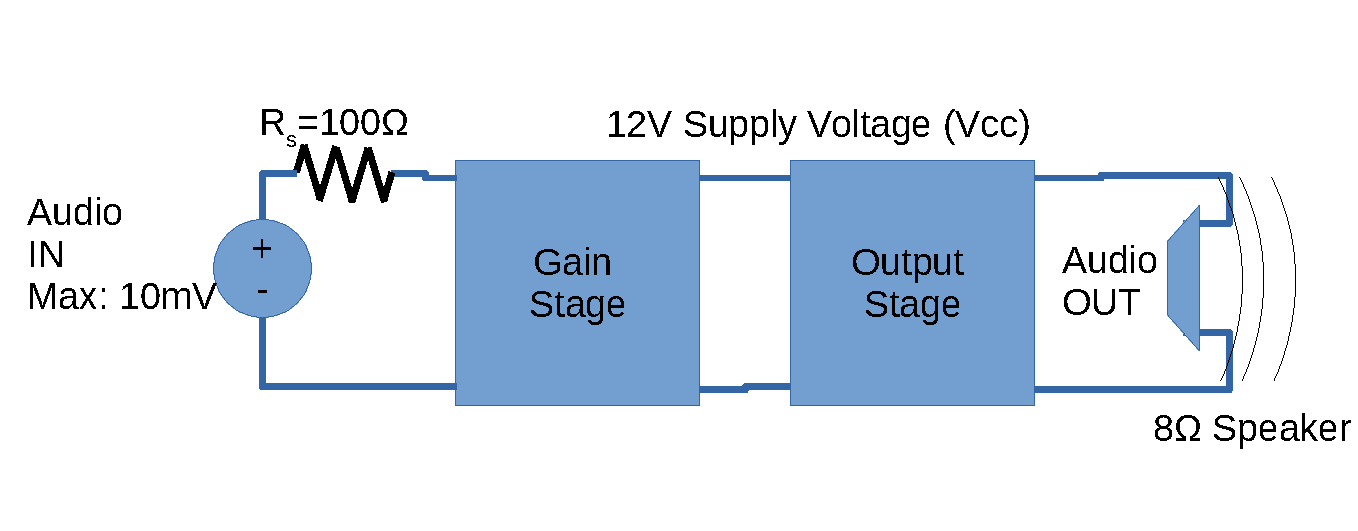
\includegraphics[width=0.8\linewidth]{amp.pdf}
\caption{Audio Amplifier Circuit}                                     
\label{fig:amp}
\end{figure}
The objective of this laboratory assignment is to simulate an Audio Amplifier Circuit as shown in Figure~\ref{fig:amp}. 

This way, we should choose the architecture of the Gain and Output amplifier stages, however, we must consider the cost of the components in the circuit. Its diagram is shown in Figure~\ref{fig:circuit}.
\begin{figure}[H] \centering
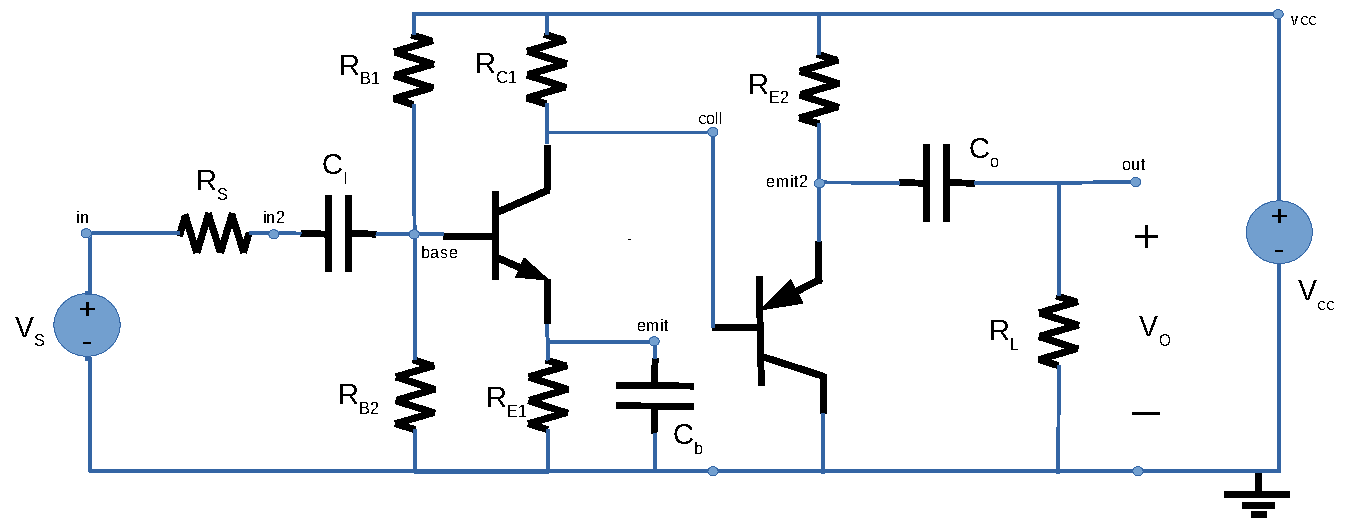
\includegraphics[width=0.8\linewidth]{circuit.pdf}
\caption{Audio Amplifier Circuit Diagram}                                     
\label{fig:circuit}
\end{figure}
In this laboratory, we use two different modles of Phillips BJT's Transistors: BC547A, a NPN transistor used in Gain Stage, and BC557A, a PNP Transistor used in Output Stage.
The values of the components are exhibited in the table below.
\begin{table}[H]
  \centering
  \begin{tabular}{|l|r|}
     \hline    
    {\bf Name} & {\bf Value} \\ \hline   
    $R_{S}$ & 1.000000e+02 Ohm\\ \hline
$R_{B1}$ & 8.000000e+04 Ohm \\ \hline
$R_{B2}$ & 2.000000e+04 Ohm \\ \hline
$R_{C1}$ & 9.400000e+02 Ohm \\ \hline
$R_{E1}$ & 7.750000e+02 Ohm \\ \hline
$R_{E2}$ & 2.335000e+03 Ohm \\ \hline
$R_{L}$ & 8.000000e+00 Ohm \\ \hline
$C_{I}$ & 6.900000e-04 F \\ \hline
$C_{b}$ & 4.180000e-03 F \\ \hline
$C_{O}$ & 2.250000e-03 F \\ \hline

  \end{tabular}
  \caption{Components Values}
  \label{tab:datags}
\end{table}

In Section~\ref{sec:analysis}, a theoretical analysis of the circuit, 
performed on Octave, is presented. In Section~\ref{sec:simulation}, the 
circuit is analysed by simulation, using NGSpice, and the results are compared to 
the theoretical results obtained in Section~\ref{sec:analysis}. The conclusions 
of this study are outlined in Section~\ref{sec:conclusion}.


